%  !TeX  root  =  user_guide.tex

\section{Interpolation Plugin}\label{sec:interpol}

% when the revision of a section has been finalized, 
% comment out the following line:
% \updatedisclaimer

The Interplation plugin can be used to generate a TIN or IDW interpolation of a 
point vector layer. It is very simple to handle and provides an intiuitive graphical 
user interface for creating interpolated raster layers (See Figure \ref{fig:interpolation_dialog}).
The plugin requires the following parameters to be specified before running:

\begin{itemize}[label=--]
\item \textbf{Input vector layer}: Specify the input point vector layer(s) from a list of loaded
point layers. If several layers are specified, then data from all layers is used for
interpolation. Note: It is possible to insert lines or polygons as constraints for the
triangulation, by specifying either ``structure lines'' or ``break lines'' in the
\dropmenuopt{Type} dropdown menu.
\item \textbf{Interpolation attribute}: Select attribute column to be used for interpolation or 
enable the \checkbox{Use Z-Coordinate} checkbox to use the layers stored Z values.
\item \textbf{Interpolation Method}: Select interpolation method. This can be either \selectstring{Triangulated Irregular 
Network (TIN)}{\ldots} or \selectstring{Inverse Distance Weighted (IDW)}{\ldots}.
\item \textbf{Number of columns/rows}: Specify the number row and colums for the output raster file.
\item \textbf{Output file}: Specify a name for the output raster file.
\end{itemize}

\begin{figure}[ht]
   \centering
   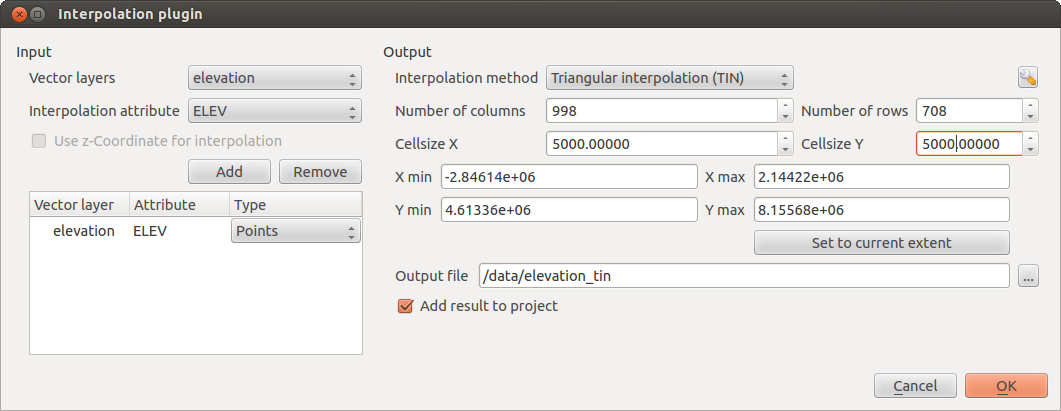
\includegraphics[clip=true, width=14cm]{interpolate_dialog}
   \caption{Interpolation Plugin \nixcaption}\label{fig:interpolation_dialog}
\end{figure}

\minisec{Using the plugin}\label{interpolation_usage}

\begin{enumerate}
  \item Start QGIS and load an point vector layer (e.g., \filename{elevp.csv}). 
  \item Load the Interpolation plugin in the Plugin Manager (see Section 
  \ref{sec:load_core_plugin}) and click on the \toolbtntwo{interpolation}{Interpolation} 
  icon which appears in the QGIS toolbar menu. The Interpolation plugin dialog appears as 
  shown in Figure \ref{fig:interpolation_dialog}.
  \item Select an input layer (e.g., \selectstring{elevp}{\ldots}) and column (e.g. \filename{ELEV}) for 
  interpolation.
  \item Select an interpolation method (e.g. \selectstring{Triangular interpolation}{\ldots}), and specify a cellsize of 5000 as well as the raster output filename (e.g., \filename{elevation\_tin}).
  \item Click \button{Ok}.
  \item For the current example, double click \filename{elevation\_tin} in the layer list to open the Raster Layer Properties 
  dialog and select \selectstring{Pseudocolor}{\ldots} as Color Map in the \tab{Symbology} tab. Or you 
  can define a new color table as described in Section \ref{label_rasterprop}.
\end{enumerate}

In Figure \ref{fig:interpolation_idw} you see the TIN interpolation result with a 998 cols x 812 rows (5 km) resolution for the \filename{elevp.csv} data visualized using the Pseudocolor color table. The processing only takes a few minutes, and covers the northern part of Alaska.

\begin{figure}[ht]
   \centering
   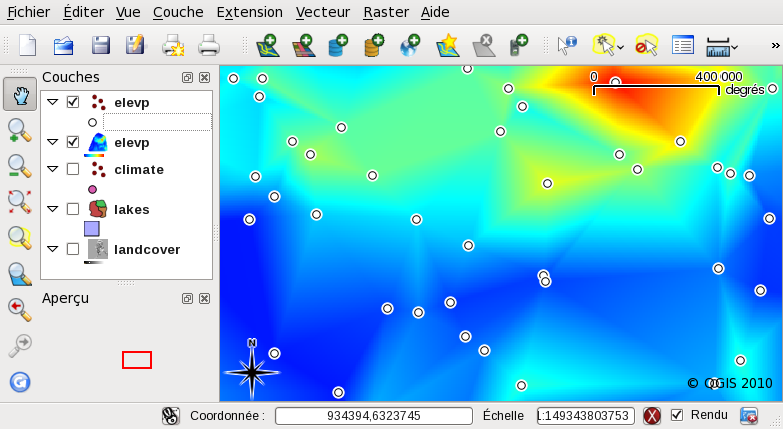
\includegraphics[clip=true, width=10cm]{interpolate_tin}
   \caption{Interpolation of elevp data using TIN method \nixcaption}\label{fig:interpolation_idw}
\end{figure}

\FloatBarrier
